% Options for packages loaded elsewhere
\PassOptionsToPackage{unicode}{hyperref}
\PassOptionsToPackage{hyphens}{url}
%
\documentclass[
  man]{apa6}
\usepackage{amsmath,amssymb}
\usepackage{iftex}
\ifPDFTeX
  \usepackage[T1]{fontenc}
  \usepackage[utf8]{inputenc}
  \usepackage{textcomp} % provide euro and other symbols
\else % if luatex or xetex
  \usepackage{unicode-math} % this also loads fontspec
  \defaultfontfeatures{Scale=MatchLowercase}
  \defaultfontfeatures[\rmfamily]{Ligatures=TeX,Scale=1}
\fi
\usepackage{lmodern}
\ifPDFTeX\else
  % xetex/luatex font selection
\fi
% Use upquote if available, for straight quotes in verbatim environments
\IfFileExists{upquote.sty}{\usepackage{upquote}}{}
\IfFileExists{microtype.sty}{% use microtype if available
  \usepackage[]{microtype}
  \UseMicrotypeSet[protrusion]{basicmath} % disable protrusion for tt fonts
}{}
\makeatletter
\@ifundefined{KOMAClassName}{% if non-KOMA class
  \IfFileExists{parskip.sty}{%
    \usepackage{parskip}
  }{% else
    \setlength{\parindent}{0pt}
    \setlength{\parskip}{6pt plus 2pt minus 1pt}}
}{% if KOMA class
  \KOMAoptions{parskip=half}}
\makeatother
\usepackage{xcolor}
\usepackage{color}
\usepackage{fancyvrb}
\newcommand{\VerbBar}{|}
\newcommand{\VERB}{\Verb[commandchars=\\\{\}]}
\DefineVerbatimEnvironment{Highlighting}{Verbatim}{commandchars=\\\{\}}
% Add ',fontsize=\small' for more characters per line
\usepackage{framed}
\definecolor{shadecolor}{RGB}{248,248,248}
\newenvironment{Shaded}{\begin{snugshade}}{\end{snugshade}}
\newcommand{\AlertTok}[1]{\textcolor[rgb]{0.94,0.16,0.16}{#1}}
\newcommand{\AnnotationTok}[1]{\textcolor[rgb]{0.56,0.35,0.01}{\textbf{\textit{#1}}}}
\newcommand{\AttributeTok}[1]{\textcolor[rgb]{0.13,0.29,0.53}{#1}}
\newcommand{\BaseNTok}[1]{\textcolor[rgb]{0.00,0.00,0.81}{#1}}
\newcommand{\BuiltInTok}[1]{#1}
\newcommand{\CharTok}[1]{\textcolor[rgb]{0.31,0.60,0.02}{#1}}
\newcommand{\CommentTok}[1]{\textcolor[rgb]{0.56,0.35,0.01}{\textit{#1}}}
\newcommand{\CommentVarTok}[1]{\textcolor[rgb]{0.56,0.35,0.01}{\textbf{\textit{#1}}}}
\newcommand{\ConstantTok}[1]{\textcolor[rgb]{0.56,0.35,0.01}{#1}}
\newcommand{\ControlFlowTok}[1]{\textcolor[rgb]{0.13,0.29,0.53}{\textbf{#1}}}
\newcommand{\DataTypeTok}[1]{\textcolor[rgb]{0.13,0.29,0.53}{#1}}
\newcommand{\DecValTok}[1]{\textcolor[rgb]{0.00,0.00,0.81}{#1}}
\newcommand{\DocumentationTok}[1]{\textcolor[rgb]{0.56,0.35,0.01}{\textbf{\textit{#1}}}}
\newcommand{\ErrorTok}[1]{\textcolor[rgb]{0.64,0.00,0.00}{\textbf{#1}}}
\newcommand{\ExtensionTok}[1]{#1}
\newcommand{\FloatTok}[1]{\textcolor[rgb]{0.00,0.00,0.81}{#1}}
\newcommand{\FunctionTok}[1]{\textcolor[rgb]{0.13,0.29,0.53}{\textbf{#1}}}
\newcommand{\ImportTok}[1]{#1}
\newcommand{\InformationTok}[1]{\textcolor[rgb]{0.56,0.35,0.01}{\textbf{\textit{#1}}}}
\newcommand{\KeywordTok}[1]{\textcolor[rgb]{0.13,0.29,0.53}{\textbf{#1}}}
\newcommand{\NormalTok}[1]{#1}
\newcommand{\OperatorTok}[1]{\textcolor[rgb]{0.81,0.36,0.00}{\textbf{#1}}}
\newcommand{\OtherTok}[1]{\textcolor[rgb]{0.56,0.35,0.01}{#1}}
\newcommand{\PreprocessorTok}[1]{\textcolor[rgb]{0.56,0.35,0.01}{\textit{#1}}}
\newcommand{\RegionMarkerTok}[1]{#1}
\newcommand{\SpecialCharTok}[1]{\textcolor[rgb]{0.81,0.36,0.00}{\textbf{#1}}}
\newcommand{\SpecialStringTok}[1]{\textcolor[rgb]{0.31,0.60,0.02}{#1}}
\newcommand{\StringTok}[1]{\textcolor[rgb]{0.31,0.60,0.02}{#1}}
\newcommand{\VariableTok}[1]{\textcolor[rgb]{0.00,0.00,0.00}{#1}}
\newcommand{\VerbatimStringTok}[1]{\textcolor[rgb]{0.31,0.60,0.02}{#1}}
\newcommand{\WarningTok}[1]{\textcolor[rgb]{0.56,0.35,0.01}{\textbf{\textit{#1}}}}
\usepackage{graphicx}
\makeatletter
\def\maxwidth{\ifdim\Gin@nat@width>\linewidth\linewidth\else\Gin@nat@width\fi}
\def\maxheight{\ifdim\Gin@nat@height>\textheight\textheight\else\Gin@nat@height\fi}
\makeatother
% Scale images if necessary, so that they will not overflow the page
% margins by default, and it is still possible to overwrite the defaults
% using explicit options in \includegraphics[width, height, ...]{}
\setkeys{Gin}{width=\maxwidth,height=\maxheight,keepaspectratio}
% Set default figure placement to htbp
\makeatletter
\def\fps@figure{htbp}
\makeatother
\setlength{\emergencystretch}{3em} % prevent overfull lines
\providecommand{\tightlist}{%
  \setlength{\itemsep}{0pt}\setlength{\parskip}{0pt}}
\setcounter{secnumdepth}{-\maxdimen} % remove section numbering
% Make \paragraph and \subparagraph free-standing
\ifx\paragraph\undefined\else
  \let\oldparagraph\paragraph
  \renewcommand{\paragraph}[1]{\oldparagraph{#1}\mbox{}}
\fi
\ifx\subparagraph\undefined\else
  \let\oldsubparagraph\subparagraph
  \renewcommand{\subparagraph}[1]{\oldsubparagraph{#1}\mbox{}}
\fi
\newlength{\cslhangindent}
\setlength{\cslhangindent}{1.5em}
\newlength{\csllabelwidth}
\setlength{\csllabelwidth}{3em}
\newlength{\cslentryspacingunit} % times entry-spacing
\setlength{\cslentryspacingunit}{\parskip}
\newenvironment{CSLReferences}[2] % #1 hanging-ident, #2 entry spacing
 {% don't indent paragraphs
  \setlength{\parindent}{0pt}
  % turn on hanging indent if param 1 is 1
  \ifodd #1
  \let\oldpar\par
  \def\par{\hangindent=\cslhangindent\oldpar}
  \fi
  % set entry spacing
  \setlength{\parskip}{#2\cslentryspacingunit}
 }%
 {}
\usepackage{calc}
\newcommand{\CSLBlock}[1]{#1\hfill\break}
\newcommand{\CSLLeftMargin}[1]{\parbox[t]{\csllabelwidth}{#1}}
\newcommand{\CSLRightInline}[1]{\parbox[t]{\linewidth - \csllabelwidth}{#1}\break}
\newcommand{\CSLIndent}[1]{\hspace{\cslhangindent}#1}
\ifLuaTeX
\usepackage[bidi=basic]{babel}
\else
\usepackage[bidi=default]{babel}
\fi
\babelprovide[main,import]{english}
% get rid of language-specific shorthands (see #6817):
\let\LanguageShortHands\languageshorthands
\def\languageshorthands#1{}
% Manuscript styling
\usepackage{upgreek}
\captionsetup{font=singlespacing,justification=justified}

% Table formatting
\usepackage{longtable}
\usepackage{lscape}
% \usepackage[counterclockwise]{rotating}   % Landscape page setup for large tables
\usepackage{multirow}		% Table styling
\usepackage{tabularx}		% Control Column width
\usepackage[flushleft]{threeparttable}	% Allows for three part tables with a specified notes section
\usepackage{threeparttablex}            % Lets threeparttable work with longtable

% Create new environments so endfloat can handle them
% \newenvironment{ltable}
%   {\begin{landscape}\centering\begin{threeparttable}}
%   {\end{threeparttable}\end{landscape}}
\newenvironment{lltable}{\begin{landscape}\centering\begin{ThreePartTable}}{\end{ThreePartTable}\end{landscape}}

% Enables adjusting longtable caption width to table width
% Solution found at http://golatex.de/longtable-mit-caption-so-breit-wie-die-tabelle-t15767.html
\makeatletter
\newcommand\LastLTentrywidth{1em}
\newlength\longtablewidth
\setlength{\longtablewidth}{1in}
\newcommand{\getlongtablewidth}{\begingroup \ifcsname LT@\roman{LT@tables}\endcsname \global\longtablewidth=0pt \renewcommand{\LT@entry}[2]{\global\advance\longtablewidth by ##2\relax\gdef\LastLTentrywidth{##2}}\@nameuse{LT@\roman{LT@tables}} \fi \endgroup}

% \setlength{\parindent}{0.5in}
% \setlength{\parskip}{0pt plus 0pt minus 0pt}

% Overwrite redefinition of paragraph and subparagraph by the default LaTeX template
% See https://github.com/crsh/papaja/issues/292
\makeatletter
\renewcommand{\paragraph}{\@startsection{paragraph}{4}{\parindent}%
  {0\baselineskip \@plus 0.2ex \@minus 0.2ex}%
  {-1em}%
  {\normalfont\normalsize\bfseries\itshape\typesectitle}}

\renewcommand{\subparagraph}[1]{\@startsection{subparagraph}{5}{1em}%
  {0\baselineskip \@plus 0.2ex \@minus 0.2ex}%
  {-\z@\relax}%
  {\normalfont\normalsize\itshape\hspace{\parindent}{#1}\textit{\addperi}}{\relax}}
\makeatother

\makeatletter
\usepackage{etoolbox}
\patchcmd{\maketitle}
  {\section{\normalfont\normalsize\abstractname}}
  {\section*{\normalfont\normalsize\abstractname}}
  {}{\typeout{Failed to patch abstract.}}
\patchcmd{\maketitle}
  {\section{\protect\normalfont{\@title}}}
  {\section*{\protect\normalfont{\@title}}}
  {}{\typeout{Failed to patch title.}}
\makeatother

\usepackage{xpatch}
\makeatletter
\xapptocmd\appendix
  {\xapptocmd\section
    {\addcontentsline{toc}{section}{\appendixname\ifoneappendix\else~\theappendix\fi\\: #1}}
    {}{\InnerPatchFailed}%
  }
{}{\PatchFailed}
\usepackage{csquotes}
\ifLuaTeX
  \usepackage{selnolig}  % disable illegal ligatures
\fi
\IfFileExists{bookmark.sty}{\usepackage{bookmark}}{\usepackage{hyperref}}
\IfFileExists{xurl.sty}{\usepackage{xurl}}{} % add URL line breaks if available
\urlstyle{same}
\hypersetup{
  pdftitle={PSYC 30550},
  pdfauthor={Sooyoun Zong},
  pdflang={en-EN},
  hidelinks,
  pdfcreator={LaTeX via pandoc}}

\title{PSYC 30550}
\author{Sooyoun Zong\textsuperscript{}}
\date{}


\shorttitle{Ses-infer project pilot RMD}

\affiliation{\phantom{0}}

\begin{document}
\maketitle

\hypertarget{hw-15-analysis-plan}{%
\subsection{HW (15) Analysis Plan}\label{hw-15-analysis-plan}}

\begin{enumerate}
\def\labelenumi{\arabic{enumi}.}
\tightlist
\item
  Independent variable Vignettes (two explanation levels X two social classes)
\end{enumerate}

\begin{itemize}
\tightlist
\item
  3 higher-class topic vignettes + 3 lower-class topic vignettes
\item
  Each vignette has basic (detailed explanation) and neutral version (no explanation)
\end{itemize}

\begin{enumerate}
\def\labelenumi{\arabic{enumi}.}
\setcounter{enumi}{1}
\tightlist
\item
  Dependent variable
\end{enumerate}

\begin{itemize}
\tightlist
\item
  Listener's knowledge rating (7-point Likert)
\item
  Listener's social class rating (10-point Likert)
\item
  Participant's social class + knowledge of various topics
\end{itemize}

\begin{enumerate}
\def\labelenumi{\arabic{enumi}.}
\setcounter{enumi}{2}
\tightlist
\item
  Analysis
\end{enumerate}

A. Relationship between participant social class and knowledge
- Analysis: Correlation analysis for manipulation check ∙ for selecting topics for future study
- Plot: Scatter plot + fitted line visualizing the relationship
- Table: Correlation matrix with correlation coefficients, significance levels

B. Compare knowledge and social class ratings between conditions
- Analysis: ANOVA (among four groups) or Independent samples t-test (between two explanation conditions) to compare (1) average knowledge ratings (2) social class ratings
- Plots: (1) Histograms visualizing the data distribution (2) Bar graph showing the distribution of ratings for each condition
- Tables: (1) Descriptive statistics of means \& standard deviations (2) Summary of ANOVA / t-test results

\hypertarget{hw-16--1-example-correlation-analyses}{%
\section{HW (16) -1 Example correlation analyses}\label{hw-16--1-example-correlation-analyses}}

\textbf{Data not collected yet}

\begin{Shaded}
\begin{Highlighting}[]
\FunctionTok{library}\NormalTok{(dplyr)}
\FunctionTok{library}\NormalTok{(ggplot2)}
\FunctionTok{library}\NormalTok{(readxl)}
\FunctionTok{library}\NormalTok{(writexl)}
\FunctionTok{library}\NormalTok{(tidyverse)}
\FunctionTok{library}\NormalTok{(citr)}
\FunctionTok{library}\NormalTok{(papaja)}

\NormalTok{dataset }\OtherTok{\textless{}{-}} \FunctionTok{read\_xlsx}\NormalTok{(}\StringTok{"dataset.xlsx"}\NormalTok{)}

\NormalTok{dataset }\SpecialCharTok{\%\textgreater{}\%}
  \FunctionTok{summarise}\NormalTok{(}
    \AttributeTok{avg\_participant\_social\_class =} \FunctionTok{mean}\NormalTok{(participant\_social\_class, }\AttributeTok{na.rm =} \ConstantTok{TRUE}\NormalTok{),}
    \AttributeTok{sd\_participant\_social\_class =} \FunctionTok{sd}\NormalTok{(participant\_social\_class, }\AttributeTok{na.rm =} \ConstantTok{TRUE}\NormalTok{),}
    \AttributeTok{sd\_knowledge =} \FunctionTok{sd}\NormalTok{(knowledge, }\AttributeTok{na.rm =} \ConstantTok{TRUE}\NormalTok{),}
    \AttributeTok{avg\_social\_class =} \FunctionTok{mean}\NormalTok{(social\_class, }\AttributeTok{na.rm =} \ConstantTok{TRUE}\NormalTok{),}
    \AttributeTok{sd\_social\_class =} \FunctionTok{sd}\NormalTok{(social\_class, }\AttributeTok{na.rm =} \ConstantTok{TRUE}\NormalTok{))}
\end{Highlighting}
\end{Shaded}

\begin{verbatim}
## # A tibble: 1 x 5
##   avg_participant_social_~1 sd_participant_socia~2 sd_knowledge avg_social_class
##                       <dbl>                  <dbl>        <dbl>            <dbl>
## 1                      4.92                   1.57        0.865             5.57
## # i abbreviated names: 1: avg_participant_social_class,
## #   2: sd_participant_social_class
## # i 1 more variable: sd_social_class <dbl>
\end{verbatim}

\begin{Shaded}
\begin{Highlighting}[]
\FunctionTok{library}\NormalTok{(psych)}

\FunctionTok{cor.test}\NormalTok{(dataset}\SpecialCharTok{$}\NormalTok{participant\_social\_class, dataset}\SpecialCharTok{$}\NormalTok{topic\_knowledge)}
\end{Highlighting}
\end{Shaded}

\begin{verbatim}
## 
##  Pearson's product-moment correlation
## 
## data:  dataset$participant_social_class and dataset$topic_knowledge
## t = 1.8869, df = 85, p-value = 0.06258
## alternative hypothesis: true correlation is not equal to 0
## 95 percent confidence interval:
##  -0.01058652  0.39449491
## sample estimates:
##       cor 
## 0.2005089
\end{verbatim}

\begin{Shaded}
\begin{Highlighting}[]
\FunctionTok{ggplot}\NormalTok{(dataset, }\FunctionTok{aes}\NormalTok{(}\AttributeTok{x =}\NormalTok{ participant\_social\_class, }\AttributeTok{y =}\NormalTok{ topic\_knowledge)) }\SpecialCharTok{+}
  \FunctionTok{geom\_point}\NormalTok{(}\AttributeTok{alpha =} \FloatTok{0.5}\NormalTok{) }\SpecialCharTok{+}
  \FunctionTok{geom\_smooth}\NormalTok{(}\AttributeTok{method =} \StringTok{"lm"}\NormalTok{, }\AttributeTok{color =} \StringTok{"blue"}\NormalTok{) }\SpecialCharTok{+}
  \FunctionTok{labs}\NormalTok{(}\AttributeTok{title =} \StringTok{"Relationship between participant social class and knowledge of topic"}\NormalTok{,}
       \AttributeTok{x =} \StringTok{"Participant social class"}\NormalTok{,}
       \AttributeTok{y =} \StringTok{"Knowledge of topic"}\NormalTok{)}
\end{Highlighting}
\end{Shaded}

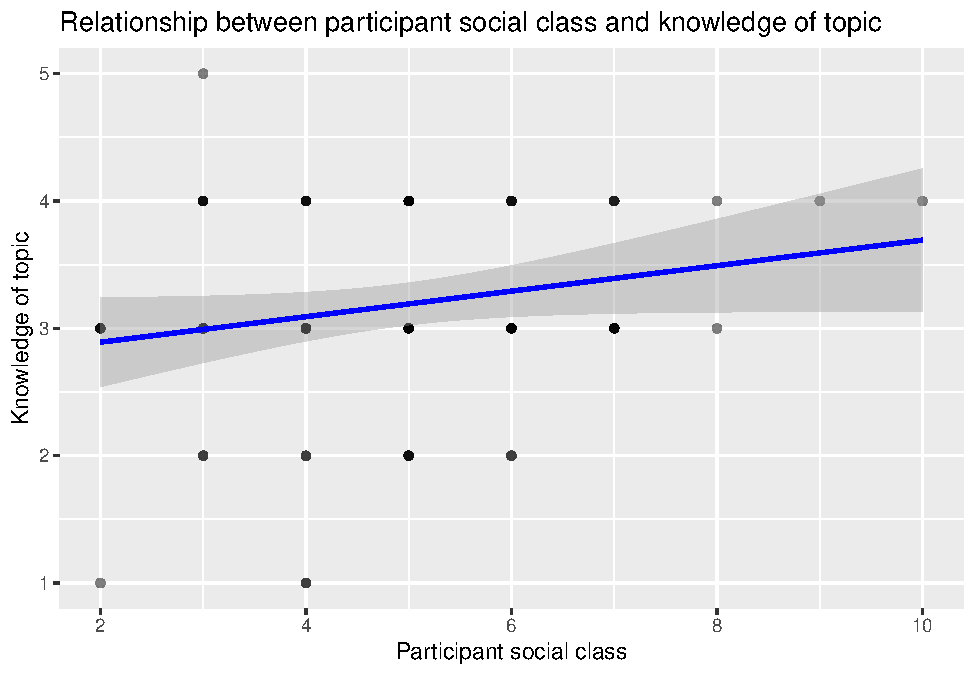
\includegraphics{sooyoun-pilot_files/figure-latex/hypothesis testing-1.pdf}

\begin{Shaded}
\begin{Highlighting}[]
\NormalTok{cor\_matrix }\OtherTok{\textless{}{-}} \FunctionTok{cor}\NormalTok{(dataset[}\FunctionTok{c}\NormalTok{(}\StringTok{"participant\_social\_class"}\NormalTok{, }\StringTok{"topic\_knowledge"}\NormalTok{)], }\AttributeTok{use =} \StringTok{"complete.obs"}\NormalTok{)}
\FunctionTok{print}\NormalTok{(cor\_matrix)}
\end{Highlighting}
\end{Shaded}

\begin{verbatim}
##                          participant_social_class topic_knowledge
## participant_social_class                1.0000000       0.2005089
## topic_knowledge                         0.2005089       1.0000000
\end{verbatim}

\hypertarget{hw-16--2-example-advanced-analysis-mixed-effects-model}{%
\section{HW (16) -2 Example advanced analysis (mixed-effects model)}\label{hw-16--2-example-advanced-analysis-mixed-effects-model}}

\hypertarget{hw-17-in-line-code-references}{%
\section{HW (17) In-line code references}\label{hw-17-in-line-code-references}}

The study explores the relationship between participants' social class and their knowledge of various conversation topics. The social class of r nrow(data) individuals was measured on a 10-point likert scale (MacArthur Subjective SES ladder), and their knowledge across different topics (that are typically well-known by either higher or lower social class group) was assessed on a 7-point likert scale.

The analyses will reveal an average participant social class of r mean(dataset\(participant_social_class, na.rm = TRUE), with a standard deviation of r sd(dataset\)participant\_social\_class, na.rm = TRUE). Knowledge on the topics will show an average score of r mean(dataset\(topic_knowledge, na.rm = TRUE), and a standard deviation of r sd(dataset\)topic\_knowledge, na.rm = TRUE).

The correlation test will indicate a significant relationship between social class and knowledge, with a correlation coefficient of r cor\_test\_result\(estimate and a p-value of r cor_test_result\)p.value. This will suggest that as participants' social class increases, their knowledge on higher-class common ground topics will also tend to increase, and vice versa.

A scatter plot will visualize this relationship with a fitted line indicating the direction and strength of the relationships. The correlation matrix will additionally reveal a coefficient of r cor\_matrix{[}``participant\_social\_class'', ``topic\_knowledge''{]}.

The findings will ultimately suggest that socioeconomic factors may indeed play a role in shaping individuals' cultivated knowledge of specific culture amd experiences.

Clark and Schreuder (1983)
Kraus, Torrez, and Park (2019)
Sebastian and Bouchard Ryan (2018)
Brown-Schmidt and Hanna (2011)
Bjornsdottir and Rule (2017)

\hypertarget{refs}{}
\begin{CSLReferences}{1}{0}
\leavevmode\vadjust pre{\hypertarget{ref-bjornsdottirVisibilitySocialClass2017}{}}%
Bjornsdottir, R. T., \& Rule, N. O. (2017). The visibility of social class from facial cues. \emph{Journal of Personality and Social Psychology}, \emph{113}(4), 530--546.

\leavevmode\vadjust pre{\hypertarget{ref-brown-schmidtTalkingAnotherPerson2011}{}}%
Brown-Schmidt, S., \& Hanna, J. E. (2011). Talking in another person's shoes: {Incremental} perspective-taking in language processing. \emph{Dialogue Discourse}, \emph{2}, 11--33.

\leavevmode\vadjust pre{\hypertarget{ref-clarkCommonGroundUnderstanding1983}{}}%
Clark, H. H., \& Schreuder, R. (1983). Common ground at the understanding of demonstrative reference. \emph{Journal of Verbal Learning and Verbal Behavior}, \emph{22}(2), 245--258.

\leavevmode\vadjust pre{\hypertarget{ref-krausEvidenceReproductionSocial2019}{}}%
Kraus, M. W., Torrez, B., \& Park, J. W. (2019). Evidence for the reproduction of social class in brief speech. \emph{Proceedings of the National Academy of Sciences of the United States of America}, \emph{116}(46), 22998--23003.

\leavevmode\vadjust pre{\hypertarget{ref-sebastianSpeechCuesSocial2018}{}}%
Sebastian, R. J., \& Bouchard Ryan, E. (2018). Speech cues and social evaluation: {Markers} of ethnicity, social class, and age. \emph{Recent Advances in Language, Communication, and Social Psychology}, 112--143.

\end{CSLReferences}


\end{document}
